%!TEX TS-program = xelatex
%!TEX encoding = UTF-8 Unicode
  

\documentclass[notitlepage]{article}

\usepackage{bibunits}
\usepackage{comment}
\usepackage{graphicx}
\usepackage{amsmath}

% processes above options
\usepackage{palatino}  %OR newcent ncntrsbk helvet times palatino
\usepackage{url}
\usepackage{footmisc}
\usepackage{endnotes}

\setlength{\parindent}{0em}
\setlength{\parskip}{1em}

\setcounter{secnumdepth}{0}
\begin{document}

\title{Bootcamp 3 - Communication Diagram}
\author{Boris Ermakov-Spektor}
\date{30 September 2019}

\maketitle

\tableofcontents

\newpage

\section{Relationships Between Files}

	\par "server.js" is just an entrypoint for "app.js", which itself
	just starts the express server in "express.js".

	\par "router.js" is used to define a routing middleware for
	express, and is used in "express.js" to handle all
	requests to /api/listings.

	\par Sequence Diagrams for every request to /api/listings are below.
	They all start at the router, after express passes control to
	the router middleware.

	\begin{center}	
		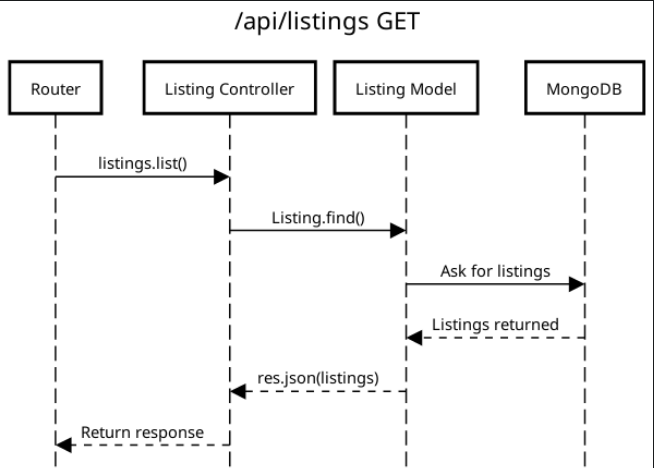
\includegraphics[width=5in]{list.png}
		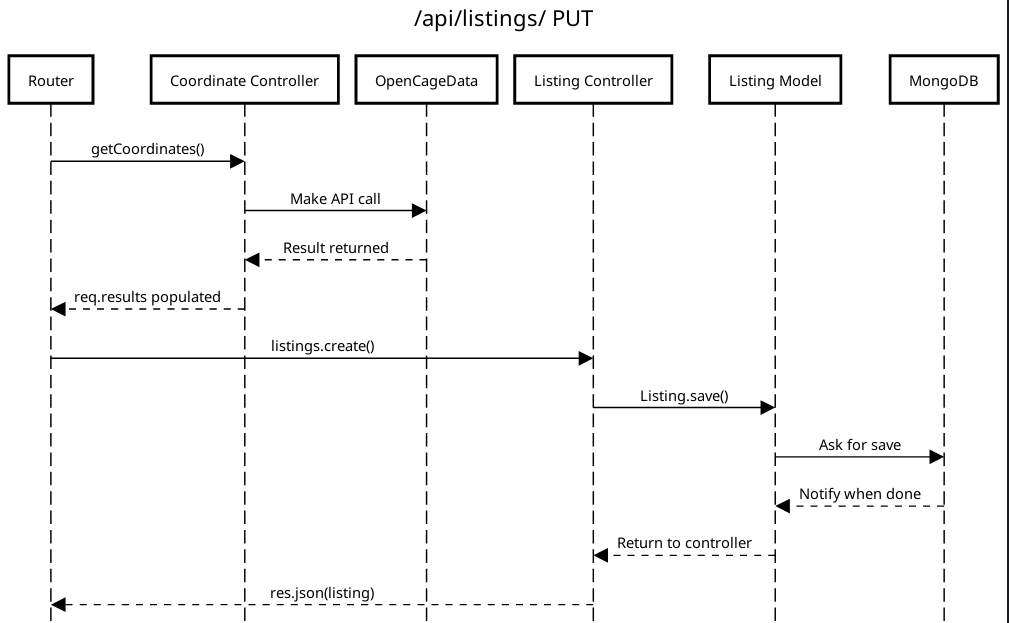
\includegraphics[width=5in]{create.png}
		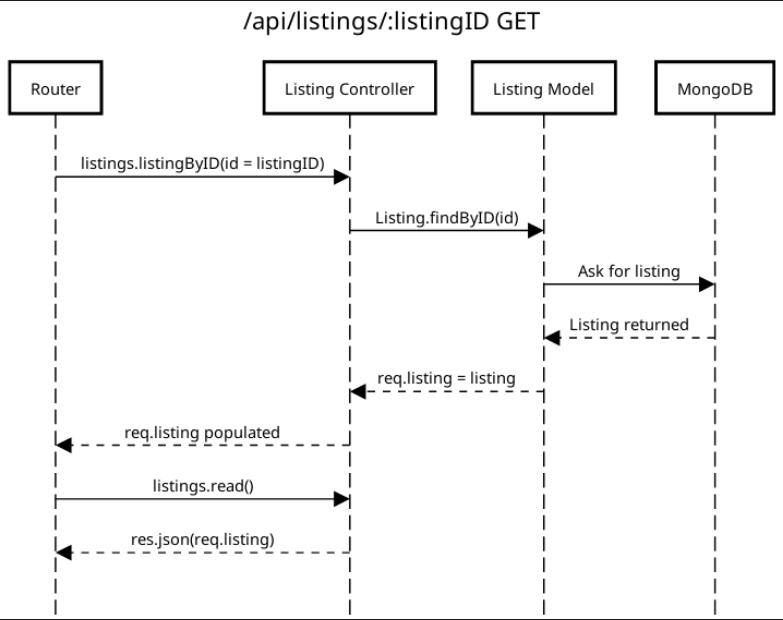
\includegraphics[width=5in]{read.png}
		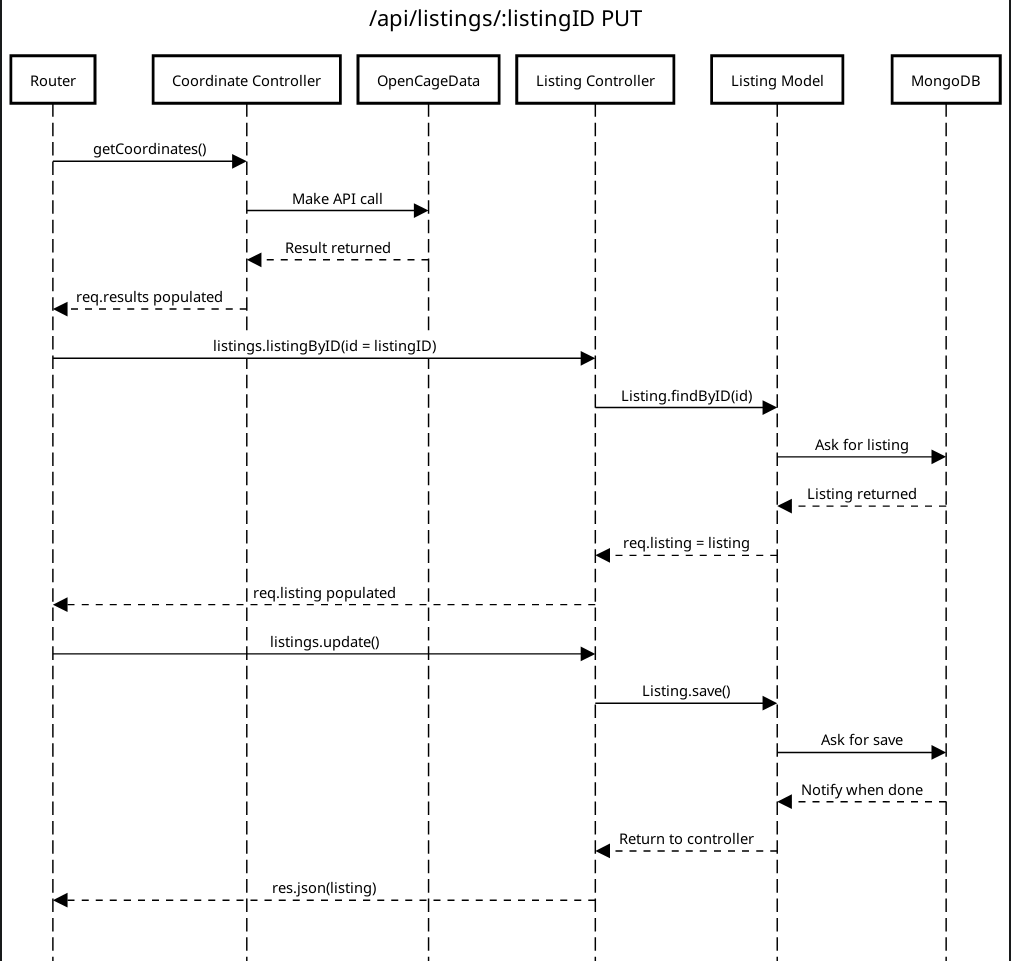
\includegraphics[width=5in]{update.png}
		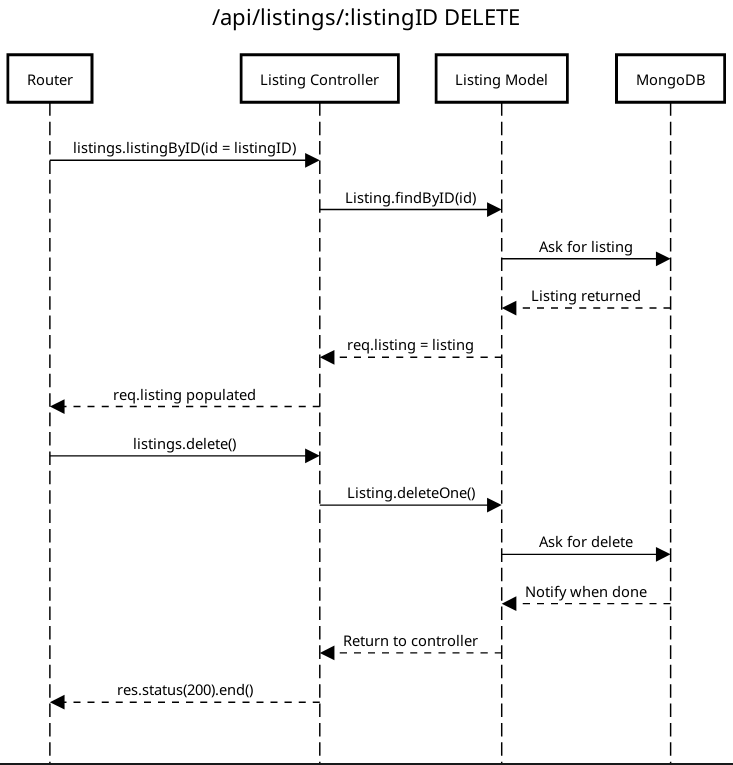
\includegraphics[width=5in]{delete.png}
	\end{center}

\section{Controller Contents And Their Roles}

	\par The coordinate controller is an implementation of a
	middleware to get coordinates from an address using an api.
	This controller is used as middleware in the router to get
	the coordinates before passing the request to the listing 
	controller.

	\par The listing controller listingByID function is another middleware
	that is used in the router to populate req.listing with the
	listing if an id is passed in before passing the request to the
	listing controller.

	\par The listing controller handles the listing requests list, create, 
	read, update, and delete.

\section{Test File Relationships}

	\par The test file "listings.server.model.test.js" tests the mongoose
	model for listings. It tells me to ensure that the name and code
	field both exist before saving the listing to MongoDB. It also
	verifies that the model properly gets saved to the database.

	\par The test file "listings.server.routes.test.js" tests the
	router, as well as both controllers. The coordinate controller is
	used as middleware inside the router, and the listings controller
	is used for the api requests inside of the router.
	The tests tell me that I need to finish the implementation of all 
	the api requests.
	It also tells me that I need to finish the coordinate controller
	implementation so that the returned coordinates get saved into
	the response at res.body.coordinates.

\end{document}
